%--------------------------------------------------
%                 P A C K A G E S
%--------------------------------------------------

\documentclass[10pt,a4paper]{article}
\usepackage[utf8]{inputenc}
\usepackage[a4paper, total={6.5in, 10in}]{geometry}
\usepackage{amsmath}
\usepackage{amsfonts}
\usepackage{amssymb}
\usepackage{hyperref}
\usepackage{graphicx}
\usepackage[export]{adjustbox}
\usepackage{subcaption}
\usepackage{hyperref}
\usepackage{fancyvrb}
\usepackage{enumitem}
\usepackage{cprotect}
\usepackage{array}

%--------------------------------------------------
%   D O C U M E N T   C O N F I G U R A T I O N
%--------------------------------------------------

\newcommand*{\pslogo}{\includegraphics{logo}}

%--------------------------------------------------
%                T I T L E P A G E
%--------------------------------------------------

\newcommand*{\dctitle}
{
	\begingroup
	\hbox
	{
		\hspace*{0.15\textwidth}
		\rule{1pt}{\textheight}
		\hspace*{0.05\textwidth}
		\parbox[b]{0.8\textwidth}
		{
			{\noindent\huge\bfseries PROJECT-SCOPES \\[0.5\baselineskip] GAME CONCEPT}\\[2\baselineskip]
			{\noindent\Large\scshape by MicroScopes \par}

			\vspace{0.5\textheight}
			%{\noindent INSERT PROJECT-SCOPES LOGO HERE!!! \par} 
			%\pslogo
		}
	}
	\endgroup
}

%--------------------------------------------------
%         D O C U M E N T   C O N T E N T
%--------------------------------------------------

\begin{document}

% titlepage
\dctitle

% table of contents
\tableofcontents

% document content
\newpage

% general game description
\section{General game description}
\noindent Project-Scopes was meant to be a simple multiplayer game in 2D with the ability to play both via the network and at a single machine. The main inspiration we can find in Curve Fever series and legendary Snake. The aim of the game is to provide fun and excitation of rivalry for the players. The game also helps in relaxing during short breaks of intellectual work. The game offers a very easy to understand rules and easy to learn basic mechanics, which means that it is an "easy to learn, hard to master" type of game. A limitation of the game is the lack of singleplayer mode. However, the side effect is gathering several people close to each other which directly influences on the development of social relationships.
\\
\\
\noindent \textbf{Main game advantages:}
\begin{itemize}
	\item[-] easy to learn game rules
	\item[-] simple control
	\item[-] direct competition
	\item[-] development of social relationships
	\item[-] minimize the impact of the random factor for the final success
\end{itemize}

% requirements for the game
\section{Requirements}

\subsection{Platform}
\noindent The target platform for Project-Scopes is a personal computer, laptop or notebook with \textbf{Windows 7} OS (or newer) and keyboard.
\subsection{Target players group}
\noindent The main target players group for Project-Scopes are bored corporats but the game is also suitable for everyone from 9 to 99 age. This game is for those who is looking for a moment of pure fun with friends. 
\subsection{Quality requirements}
\noindent Main quality requirements for Project-Scopes is minimal working resolution of \textbf{800x600px} and stable \textbf{60fps}.

% structure of the game
\section{Game structure}

\subsection{Game modes}
\noindent Project-Scopes offers two main game modes:
\begin{itemize}
	\item[-] \textbf{local mode} - in this mode, players are playing on single machine and using the same controller. Each player is involved in the game in real time and watching the game with exactly the same perspective as others (the image is not splitted).
	\item[-] \textbf{LAN mode} - in this mode player has the ability to connect to the game via the LAN network from a different, separate machine with its own controller and display. Players connected in this way are still participating in the game simultaneously in real time. Image generated for the players is the same, and it is broadcasted on their local displays.
\end{itemize}

\subsection{Interface}

\subsubsection{Menu}
\noindent Main menu appears after game starts. It offers the possibility to choose the game mode and, depending on the mode selected, the ability to set the configuration parameters of the players and the game itself.

\subsubsection{Screens}
\noindent The main screens, making up the game, are:
\begin{itemize}
	\item[-] \textbf{menu screen} - allows to choose a game mode
	\item[-] \textbf{configuration screen} - allows to set available gameplay parameters in selected mode
	\item[-] \textbf{wait for players screen} - in LAN mode means that player is ready for a game and waits for other players
	\item[-] \textbf{gameplay screen} - shows the actual gameplay
	\item[-] \textbf{pause screen} - can be launched from gameplay screen, means that the game is paused and waits for resume or close
	\item[-] \textbf{next round screen} - shows the winner of the round
	\item[-] \textbf{game over screen} - shows a table of players and points for each player position after last round end
\end{itemize}
\subsubsection{Controls}
\noindent One player needs two controller buttons to play.

\newpage
\subsection{Flowboard}
\begin{center}
	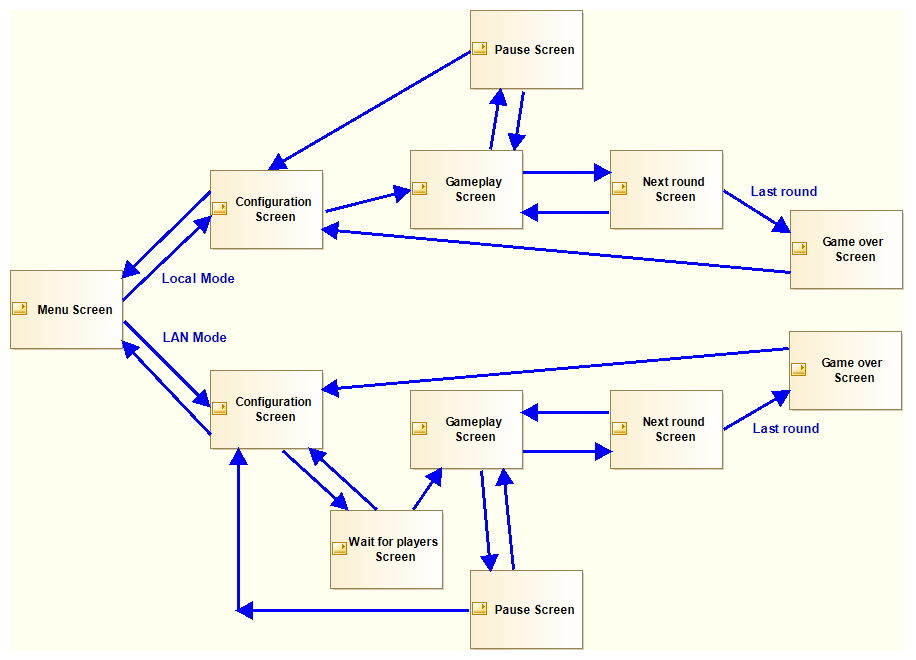
\includegraphics[width=\textwidth]{flowboard}
\end{center}

% gameplay
\section{Gameplay}
\noindent This chapter presents the general rules of the gameplay, the end game conditions and the ability to modify the basic mechanics both before and during the game. This is an information about the basic version of the game, the final version can be extended with additional elements.

\subsection{Gameplay configuration}
\noindent Options configurable from the menu screen (can't be changed during the game).
\\
\\
\noindent \textbf{Individual settings:}
\begin{itemize}
	\item[-] individual control keys for each player
	\item[-] individual color of each player (6 colors available)
	\item[-] individual nickname for each player
\end{itemize}

\noindent \textbf{Global settings:}
\begin{itemize}
	\item[-] number of players (2 - 6)
	\item[-] initial size of players
	\item[-] initial speed of players
	\item[-] initial arena size
\end{itemize}

\subsection{Main rules}
\noindent Basic (not modified) game rules:
\begin{itemize}
	\item[1.] The minimum number of players participating in the game is 2.
	\item[2.] The maximum number of players participating in the game is 6.
	\item[3.] Players plays simultaneously on a shared arena.
	\item[4.] During the game each player is moving with a constant speed in a given direction, which can be changed of specific angle by the control keys.
	\item[5.] The game is divided into rounds.
	\item[6.] The aim of the round is to eliminate the other players.
	\item[7.] A player is eliminated if he touched a trace left by another player or himself.
	\item[8.] Player can navigate only on the empty arena space between the traces of other players or its own.
	\item[9.] The player who looses the first, receives 0 points, the next eliminated player gets 1 point more than the previous one.
	\item[10.] When there only one player remains on the arena, the round is considered as complete and this player is the winner of the round. This is followed by resetting the score and start the next round.
\end{itemize}
\noindent
\\
\noindent Ending conditions:
\begin{itemize}
	\item[1.] If after the end of the round the highest total score of at least one player from all rounds is greater than or equal the winning number of points, that player is the winner of the game.
	\item[2.] The tie is possible in a situation where more than one player has the same sum of points fulfilling the condition 1.
\end{itemize}

\subsection{Gameplay modifiers (Bonuses)}
\noindent The game includes a system of bonuses that affect the basic mechanics during the game. A single bonus is an object randomly choosen from the pool of available bonuses and placed at a random moment of the game in a random place on the arena. It is represented by the corresponding graphics. If the player collides with bonus object, it disappears and activates an effect corresponding to the bonus. This effect modifies the basic mechanics and rules of the game for a certain period of time for a specific group of players. Bonus effects can accumulate or compensate each other.
\\
\\
\noindent Basic bonuses:
\begin{itemize}
	\item[-] \textbf{speed} - for a short while increases the movement speed of the player
	\item[-] \textbf{slow} - for a short while decreases the movement speed of the player
	\item[-] \textbf{thick} - for a short while increases the trace size of the player
	\item[-] \textbf{thin} - for a short while decreases the trace size of the player
	\item[-] \textbf{90 degrees} - for a short while causes the player can performs only turns by 90 degrees
\end{itemize}
\noindent Each of the bonuses described above occurs in two versions, global and individual.
\begin{itemize}
	\item[-] \textbf{Individual bonus} - it means that the effect applies only to the player who first activated the bonus
	\item[-] \textbf{Global bonus} - it means that the effect applies to all active players in the arena except the player who activated the bonus
\end{itemize}

\subsection{Game over}
\noindent When either of the ending conditions is reached, the game goes to the summary screen which displays score for all players participating in the game. The player with the highest number of points is in the first place. Next are the players who achieved the lowest results. Summary screen offers the possibility to return to the setup screen of each mode to start the next game, change the settings or mode.


% list of all images
\newpage
\listoffigures
\listoftables

\end{document}